\documentclass[11pt, english]{book}
%\usepackage[latin1]{inputenc}
\usepackage[T1]{fontenc}
\usepackage[utf8]{inputenc}
\usepackage[english]{babel}   % S P R A A K
% \usepackage{graphicx}    % postscript graphics
\usepackage{amssymb, amsmath, amsthm} % symboler, osv
\usepackage{mathrsfs}
\usepackage{url}
\usepackage{thmtools}
\usepackage{enumerate}  % lister $  
\usepackage{float}
\usepackage{tikz}
\usepackage{tikz-cd}
\usetikzlibrary{calc}
%\usepackage{tikz-3dplot}
\usepackage{subcaption}
\usepackage[all]{xy}   % for comm.diagram
\usepackage{wrapfig} % for float right
\usepackage{hyperref}
\usepackage{mystyle} % stilfilen      

%\usepackage[a5paper,margin=0.5in]{geometry}


\begin{document}
\title{All of it}
\author{Fredrik Meyer}
\maketitle 

\chapter{Preliminary definitions}

We work over $\C$. 

\section{Stanley-Reisner basics}

Given a simplicial complex $\K$, one can associate to it a projective scheme $\PP(\K)$ defined as follows. Let $P$ be the polynomial ring with one variable for each vertex of $\K$. Then the \emph{Stanley-Reisner ideal $I_\K$} corresponding to $\K$ is generated by the monomials corresponding to \emph{non-faces} of $\K$. Then we define the \emph{Stanley-Reisner scheme} to be $\Proj P/I_\K$. 

\begin{example}
Let $\K$ be the square, with vertices $v_0,v_1,v_2,v_3$. Then the Stanley-Reisner ideal is generated by $v_0v_2$ and $v_1v_3$.
\end{example}

Some of the topology of the simplicial complex is encoded in the scheme structure of $\PP(\K)$. In particular, the simplicial (co)homology groups of $\K$ can be computed as the sheaf cohomology of $\PP(\K)$

\begin{lemma}
Let $H^i(K;\C)$ denote the singular cohomology groups of $\K$. Then there are isomorphisms $H^i(K;\C)=H^i(\PP(\K),\OO_{\PP(\K)})$ for all $i$.
\end{lemma}
\begin{proof}
---------to come-----------
\end{proof}

\section{Calabi-Yau basics}

\begin{defi}
A \emph{Calabi-Yau variety} is a smooth projective variety satisfying the following two conditions:
\begin{enumerate}
	\item $H^i(X,\OO_X)=0$ for $0 < i < \dim X$.
	\item The canonical sheaf is trivial: $\omega_X \simeq \OO_X$. 
\end{enumerate}
\end{defi}

The classical example of a Calabi-Yau manifold is the quintic threefold in $\PP^5$. Another example is the following:

\begin{example}
Let $X$ be the double cover of $\PP^3$ ramified along a smooth octic. The projection map is affine, so the conditions on $H^i(X,\OO_X)$ are fulfilled. To see that the canonical sheaf is trivial, we use the adjunction formula, which says that $K_X= 2 \restr{K_{\PP^3}}{X} + \deg R$, where $R$ is the ramification divisor. Then, since $\omega_{\PP^3}=\OO_{\PP^3}(-4)$, it follows that $K_X=0$.
\end{example}

If $\K$ is a simplicial sphere, then a smoothing of $\PP(\K)$ will give a Calabi-Yau manifold. 

---- ref: bayer-eisenbud graph curves.

\section{Deformation theory}

%%%%%%%%%%%%%%%%%%%%
\chapter{Two topologically distinct smoothings}

Denote by $dP_6$ the del Pezzo surface of degree 6 embedded in $\PP^6$. This can be realized as the blow-up of $\PP^2$ in three points not lying on a line. Let $X$ denote the affine cone over $dP_6$. Then it has long been known that $X$ has two smoothing components, and we show here that they are topologically distinct.

Recall that a \emph{del Pezzo} surface is a surface such that the anti-canonical bundle is ample. The degree is the degree given by the anticanonical embedding. It is a classical result that every del Pezzo surface is obtained either by blowing up $\PP^2$ in $r=0,\ldots,6$ points in suitable positions, or as the $2$-uple embedding of a quadric surface in $\PP^3$. 

\section{Different embeddings of $dP_6$}

We first obtain the equations of $dP_6$ directly from the description of it as blow-up. Let $x_0,x_1,x_2$ be coordinates of $\PP^2$. Recall that the blowup of $\PP^2$ in the point $(1:0:0)$ can be realized as the closed subscheme of $\PP^2 \times \PP^1$ given by the equation $r_0x_1-r_1x_2=0$, where $r_0,r_1$ are coordinates on $\PP^1$. We can repeat this process on the points $(0:1:0)$ and $(0:0:1)$ to obtain similar equations. Collecting these, we see that $dP_6$ is given by the matrix equation
\[
M\vec x = 
\begin{pmatrix}
0 & r_0 & -r_1 \\
s_1 & 0 & -s_0 \\
-t_0 & t_1 & 0
\end{pmatrix}
\begin{pmatrix}
x_0 \\ y_0 \\ z_0
\end{pmatrix}= 0.
\]
in $\PP^2 \times \PP^1 \times \PP^1 \times \PP^1$. Here $r_i,s_i$ and $t_i$ ($i=0,1$) are of course coordinates on $\PP^1$.

We can do more than this however. 

\begin{lemma}
We can also realize $dP_6$ embedded in $\PP^1 \times \PP^1 \times \PP^1$ with equation $r_0s_0t_0=r_1s_1t_1$.
\end{lemma}
\begin{proof}
Note that the matrix cannot have rank $1$ or lower.

Now consider the projection onto the last three factors:
$$
\pi:\PP^2 \times \PP^1 \times \PP^1 \times \PP^1 \to \PP^1 \times \PP^1 \times \PP^1.
$$
Each point $P$ in the product on the right-hand side gives a matrix $M_P$ of rank $2$. Thus there is a line of solutions, which correspond exactly to a point in $\PP^2$.

Hence the restriction of $\pi$ to $dP_6$ is an isomorphism onto the hypersurface given by $\det M=0$ in $\PP^1 \times \PP^1 \times \PP^1$. 
\end{proof}

Another way to realize blow-ups is this: let $\mathfrak d$ be the linear system of quadrics with assigned basepoints $(1:0:0)$, $(0:1:0)$ and $(0:0:1)$ in $\PP^2$. We can choose a basis given by $x_0x_1,x_0x_2$ and $x_1x_2$. This gives a rational map $\PP^2 \rmap \PP^2$. The closure of the graph of this map is a subvariety of $\PP^2 \times \PP^2$ defined by two bilinear equations. Each of the projections correspond to the blowup.

Explicitly, if we let $y_0,y_1,y_2$ be coordinates on the other $\PP^2$, then the equations are $x_1y_0-x_1y_1=x_1y_1-x_2y_2=0$.

We also have a natural embedding in $\PP^6$ as follows. Denote by $E_1, E_2, E_3$ the exceptional divisors on the blowup. Let $L$ be a line in $\PP^2$. Then the divisor $\pi^\ast 3L - E_1-E_2-E_3$ is ample, and gives an embedding in $\PP^6$ (see \cite[Chapter V, Theorem 4.6]{hartshorne}). A basis for the corresponding linear system is given by all monomials in $\Gamma(\PP^2,\OO_{\PP^2}(3))$ except $x^3,y^3$ and $z^3$. 

The equations can be arranged in a particularly symmetric form: let $y,x_1,\ldots,x_1$ be coordinates on $\PP^6$. Then the equations of $dP_6$ are the $2 \times 2$ minors of the matrix
$$
\begin{pmatrix}
x_1 & y & x_6 \\
x_2 & x_3 & y \\
y & x_4 & x_5
\end{pmatrix}.
$$
This gives $9$ equations, which can be compactly written as $x_ix_{i+2}-yx_i=0$ and $x_ix_{i+3}-y^2=0$, for $i=1,\ldots,6$ (where $i$ is taken modulo $6$). Note that the equations have a visible $D_6$-symmetry, where $D_6$ denotes the dihedral group.

\subsection{As a toric variety}

There is a nice combinatorial description of $dP_6$ as a toric variety associated to a polytope. Namely, let $P$ denote the hexagon in \figref{hexagon}. Then the normal fan of this polytope defines a fan in $N_\R$, defining a toric variety.

\begin{figure}
\centering
\begin{subfigure}{.4 \textwidth}
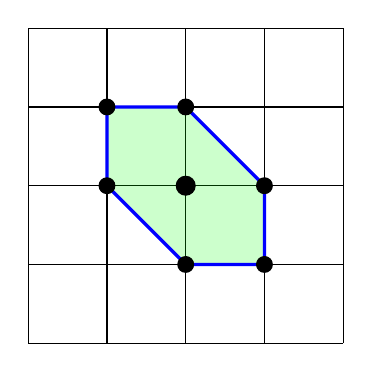
\begin{tikzpicture}
  \draw (0, 0) grid (4, 4);  

\draw [very thick, color=blue, fill=green, fill opacity=0.2]
(2,1) -- (3,1) -- (3,2) -- (2,3) -- (1,3) -- (1,2) -- cycle;

\draw [fill=black]  (2, 1) circle (0.1);
\draw [fill=black]  (3, 1) circle (0.1);
\draw [fill=black]  (3, 2) circle (0.1);
\draw [fill=black]  (2, 3) circle (0.1);
\draw [fill=black]  (1, 3) circle (0.1);
\draw [fill=black]  (1, 2) circle (0.1);
\draw [fill=black]  (2, 2) circle (0.12);
\end{tikzpicture}
\caption{The hexagon.}
\label{fig:hexagon}
\end{subfigure}
\begin{subfigure}{.4 \textwidth}
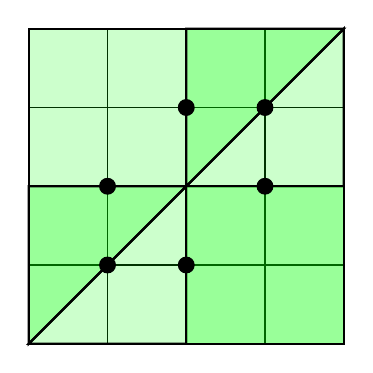
\begin{tikzpicture}
  \draw (0, 0) grid (4, 4);  
%\draw [very thick, fill=green, fill opacity=0.2]
%(1,1) -- (2,1) -- (3,2) -- (3,3) -- (2,3) -- (1,2) -- cycle;
\draw [thick,fill=green, fill opacity=0.2] (2,2) -- (4,2) -- (4,4) -- cycle;
\draw [thick,fill=green, fill opacity=0.4] (2,2) -- (4,4) -- (2,4) -- cycle;
\draw [thick,fill=green, fill opacity=0.2] (2,2) -- (2,4) -- (0,4) -- (0,2) -- cycle;
\draw [thick,fill=green, fill opacity=0.4] (2,2) -- (0,2) -- (0,0) -- cycle;
\draw [thick,fill=green, fill opacity=0.2] (2,2) -- (0,0) -- (2,0) -- cycle;
\draw [thick,fill=green, fill opacity=0.4] (2,2) -- (2,0) -- (4,0) -- (4,2) -- cycle;

\draw [fill=black]  (1, 1) circle (0.1);
\draw [fill=black]  (2, 1) circle (0.1);
\draw [fill=black]  (3, 2) circle (0.1);
\draw [fill=black]  (3, 3) circle (0.1);
\draw [fill=black]  (2, 3) circle (0.1);
\draw [fill=black]  (1, 2) circle (0.1);
%\draw [fill=black]  (2, 2) circle (0.1);
\end{tikzpicture}
\caption{The fan of $dP_6$.}
\label{fig:fandp6}
\end{subfigure}
\end{figure}

The polytope is reflexive, implying that the normal fan of $P$ is the face fan over the same polytope. See \figref{fandp6}. From standard toric geometry, it is clear that $dP_6$ is the blowup of $\PP^2$ in the three torus-fixed points. 

\section{The affine cone}

% singular at one points, deforms, balbabla 

\section{The two smoothings}

%% describe the two smoothings and prove that they are different

%%%%%%%%%%%%%%%%%%%%%%
\chapter{A smooth Calabi-Yau}

Consider the hexagon $E_6$. The join $E_6 \ast E_6$ is a $3$-dimensional sphere, and so a smoothing of the corresponding Stanley-Reisner scheme would correspond to a smooth Calabi-Yau manifold. In this chapter I prove that there does indeed exist a smoothing, and I describe some of its properties.




\bibliographystyle{plain}
\bibliography{bibliografi}

\end{document}